%This is the second chapter of the dissertation

%The following command starts your chapter. If you want different titles used in your ToC and at the top of the page throughout the chapter, you can specify those values here. Since Columbia doesn't want extra information in the headers and footers, the "Top of Page Title" value won't actually appear.

\pagestyle{cu}
\graphicspath{{./Chapter2/images/}}

\chapter[Liquid Xenon and Dual-Phase TPCs][Liquid Xenon and Dual-Phase TPCs]{Liquid Xenon and Dual-Phase TPCs}
\label{chap:lxe}

This chapter will focus on liquid xenon as a detector medium.  In \secref{sec:lxe_chem_properties} we will discuss the general properties of liquid xenon along with some of the benefits and considerations of these properties.  In \secref{sec:energy_deposition} we will discuss how charged particles in xenon deposit their energy.  In \secref{sec:lxe_er} we will discuss the production of observable light and charge from electron recoils while in \secref{sec:lxe_nr} we will discuss observable production from elastic nuclear recoils.  Finally, in \secref{sec:lxe_tpc}, we will discuss how these observables are detected in dual-phase xenon time projection chambers.

\section{General Properties}
\label{sec:lxe_chem_properties}

Xenon, with an atomic number of 54, is a noble gas meaning that it has a full valence electron shell.  Because of the full valence shell, xenon is very unlikely to interact chemically with other elements and molecules.  Xenon is also the heaviest noble gas that is, for practical purposes, naturally non-radioactive --- an essential quality for a detector medium as long-lived radioactive isotopes would be a source of background that would be very difficult to remove.  \ce{^{136}Xe}, with a natural abundance of 8.857\%, has been show to undergo double beta decay with a half-life of $2.165 \cdot 10^{21}$ years so strictly speaking natural xenon is radioactive although this process is extremely rare and has little relevance for even low background dark matter experiments \cite{albert2014improved}.  However, we will still discuss the implications of  \ce{^{136}Xe} with respect to our electronic recoil background in \secref{sec:xe1t_radioxenon}.

While natural xenon is not radioactive, it is actually possible to excite xenon nuclei such that they decay and emit gamma rays.  None of these excited states have very long lifetimes that would cause issues for low background experiments but two of these neutron activated states (\ce{^{131m}Xe} and \ce{^{129m}Xe} which decay emitting 164 keV and 236 keV photons, respectively) have half-lives on the order of ten days.  This excited states be very useful in the calibration of large detectors since over this period of time the excited states would be approximately uniformly distributed inside of a detector \cite{ni2007preparation} --- these neutron activated states are used as one of the many sources used for calibrations in XENON1T which will be discussed in \secref{sec:xe1t_calibrations}.

\begin{figure}[t]
	\centering
	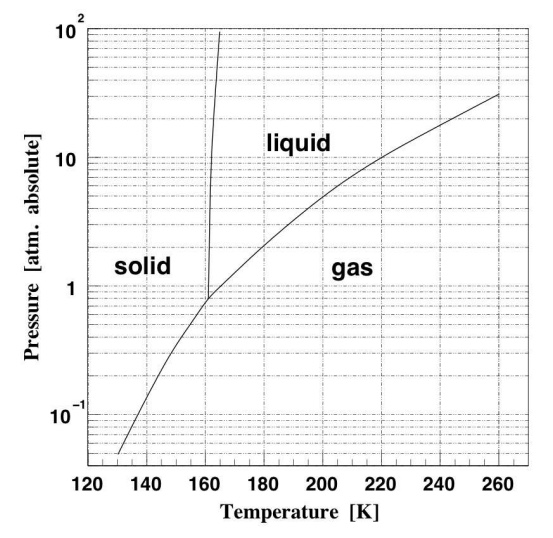
\includegraphics[width=0.7\textwidth]{xe_pt_diagram}
	\caption{The phase diagram for xenon.  Dual-phase xenon TPCs typically operate in the range of 2--3 atm.}
	\label{fig:xe_phase_diagram}
\end{figure}

Xenon is extracted from the atmosphere as a byproduct of the separation of oxygen and nitrogen.  Once the oxygen is separated, it will contain trace amounts of krypton and xenon that can be separated out further by distillation or adsorption.  The xenon that is purchased commercially typically will have a final Kr/Xe ratio of $\sim 10^{-6} - 10^{-9} \frac{\textrm{mol}}{\textrm{mol}}$.  Natural krypton is not radioactive on a relevant time scale but \ce{^{85}Kr}, which is released into the atmosphere via nuclear fuel reprocessing and nuclear weapons tests, beta decays with a mean energy of 251 keV and with a half-life of roughly 10.8 years \cite{abe2009distillation}.  So while natural xenon is not radioactive, the process of extracting xenon from the atmosphere does leave a radioactive isotope that could be a potential source of background for dark matter experiments.  Significant effort has gone into reducing the Kr/Xe levels to reduce this background as much as possible.  In XENON1T, the lowest level to date was achieved with a natural krypton to xenon ratio of less than 200 ppq (1 ppq = $10^{-15} \frac{\textrm{mol}}{\textrm{mol}}$) \cite{aprile2017removing}.



\begin{table}[t]
\centering
\label{tab:xe_abundance}
\def\arraystretch{1.3}
\begin{tabular}{ccccc}
\hline
Isotope & Abundance & Spin & Half-life & Decay Mode  \\ \hline
\ce{^{124}Xe} & 0.095\% & 0 & $ > 1.6 \cdot 10^{14}$ y & $2 \nu \beta^+ \beta^+$ \cref{fn:predicted_decay} \\ %\hline
\ce{^{126}Xe}&  0.089\% & 0 & $ 4.7 - 12 \cdot 10^{25}$ y & $2 \nu \beta^- \beta^-$ \cref{fn:predicted_decay} \\ %\hline
\ce{^{128}Xe}&  1.910\% & 0 & Stable & - \\ %\hline
\ce{^{129}Xe}&  16.400\% & $\sfrac{1}{2}$ & Stable & - \\ %\hline
\ce{^{130}Xe}&  4.071\% & 0 & Stable & - \\ %\hline
\ce{^{131}Xe}&  21.232\% & $\sfrac{3}{2}$ & Stable & - \\ %\hline
\ce{^{132}Xe}&  26.909\% & 0 & Stable & - \\ %\hline
\ce{^{134}Xe} & 10.436\% & 0 & $ > 5.8 \cdot 10^{22}$ y & $2 \nu \beta^- \beta^-$ \cref{fn:predicted_decay} \\ %\hline
\ce{^{136}Xe}&  8.857\% & 0 & $2.2 \cdot 10^{21}$ y & $2 \nu \beta^- \beta^-$ \\ %\hline
\end{tabular}
\caption{Abundances, half-lives, and decay modes of various xenon isotopes.  Note that \ce{^{136}Xe} is the only isotope whose decay has been measured.  Half-life data: \cite{barros2014double}.}
\end{table}
\stepcounter{footnote}



Dual-phase xenon experiments typically operate at roughly 2--3 atm, which translates to a boiling point of roughly 180 K ($-93.2^{\circ}$ C).  The density of liquid xenon (LXe) at this temperature is roughly 2.84 g/$\textrm{cm}^3$ which is significantly higher than all of the other noble elements, with the exception of radon \cite{rankin2009crc}.  The high density of LXe is partly responsible for its high electronic stopping power, which will be discussed further in the next section.





\section{Energy Deposition of Charged Particles in Liquid Xenon}
\label{sec:energy_deposition}

Both nuclear and electronic recoils, which will be discussed in the following sections, ultimately result in a charged particles traversing the LXe - in the case of an electronic recoil the resulting charged particle is an electron and in the case of nuclear recoils it is the xenon nucleus.  Given the high density and atomic number of xenon, the electronic stopping power is large for both electrons and xenon ions ($\sim 1-30 \, \sfrac{\textrm{keV}}{\mu \textrm{m}}$).  This means that the tracks of low energy electronic and nuclear recoils will be very small and approximately point-like \cite{aprile2006simultaneous}.  In this section, we will discuss the process by which these electronic and nuclear recoils produce light and charge that can ultimately be detected in liquid xenon TPCs.  A visual diagram of these mechanisms is shown in \figref{fig:diagram_energy_deposition}.

\begin{figure}[t]
	\centering
	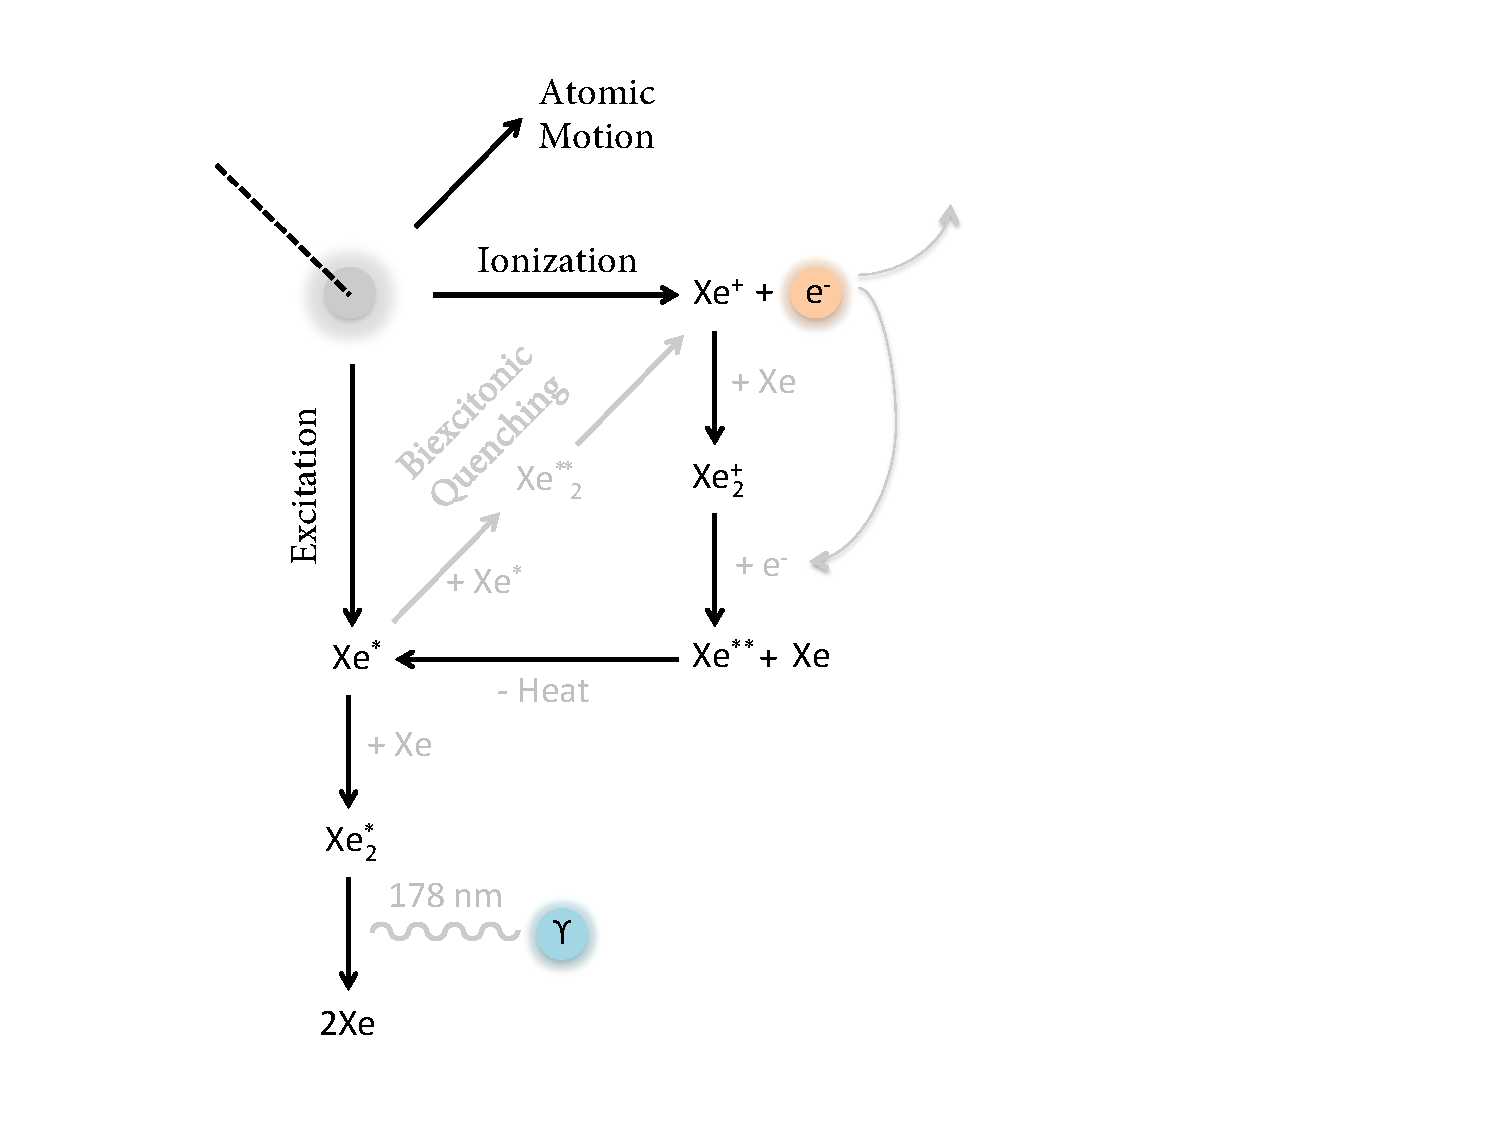
\includegraphics[width=0.7\textwidth]{observables_diagram}
	\caption{A diagram showing the modes in which charged particles may lose energy in liquid xenon.  Note that when an electric field is applied, the electron freed during ionization can be extracted such that it can be measured.}
	\label{fig:diagram_energy_deposition}
\end{figure}


In liquid xenon (and other noble liquids), scintillation light is produced via the excitation of atomic electrons and the ionization and subsequent recombination of free electrons and ions.  The excitation scintillation process is shown in \eqnref{eqn:exciton_production} and the ionization scintillation process is shown in \eqnref{eqn:ionization_production}.  


% foot note for table
\footnotetext{\label{fn:predicted_decay}This decay is predicted but has not yet been observed.}

\begin{equation}
        \label{eqn:exciton_production}
        \begin{gathered}
                \textrm{Xe*} + \textrm{Xe} + \textrm{Xe} \rightarrow \textrm{Xe*}_2 + \textrm{Xe}, \\
                \textrm{Xe*}_2 \rightarrow 2\textrm{Xe} + h \nu
        \end{gathered}
\end{equation}


\begin{equation}
        \label{eqn:ionization_production}
        \begin{gathered}
                \textrm{Xe}^+ + \textrm{Xe} \rightarrow \textrm{Xe}_2^+, \\
                \textrm{Xe}_2^+ + e^- \rightarrow \textrm{Xe**} + \textrm{Xe}, \\
                \textrm{Xe**} \rightarrow \textrm{Xe*} + \textrm{heat}, \\
                \textrm{Xe*} + \textrm{Xe} + \textrm{Xe} \rightarrow \textrm{Xe*}_2 + \textrm{Xe}, \\
                \textrm{Xe*}_2 \rightarrow 2\textrm{Xe} + h \nu
        \end{gathered}
\end{equation}

The excitation process proceeds when an an atomic electron in xenon is excited (the excited xenon is referred to as an \textit{exciton}) and the excited atom forms a dimer with another xenon atom, which is called an \textit{excimer}.  This excited excimer can be formed in either the singlet state (spin of excited electron anti-parallel to electron originally sharing state) or triplet state (spin of excited electron parallel to electron originally sharing state).  The excimers in the singlet and triplet states each have their own characteristic lifetimes (roughly 4 ns and 22 ns)\footnote{In xenon the difference in lifetimes of the singlet and triplet states is fairly small but for argon the singlet lifetime is 7 ns while the triplet lifetime is 1.3 $\mu$s \cite{heindl2011table}!} and decay into xenon atoms and a 178 nm photon (the photon falls in UV portion of the spectrum) \cite{hitachi1983effect, doke2002absolute}.  

The ionization process begins when a charged particle ionizes a xenon atom, leaving singly-ionized xenon and a free electron.  The singly-ionized xenon atom can then form an ionized dimer and subsequent excited xenon state.  This excited xenon state leads to an excimer through non-radiative heat loss.  The excimer produces scintillation light in the manner described above.

% mention charge signal
Implicit in the ionization process outlined above is the assumption that the electron freed during ionization recombines with the singly-ionized dimer.  However, in the presence of an electric field, this recombination can be reduced such that a charge signal can also be read out in addition to the scintillation signal.  Incomplete recombination can also occur at zero electric field and these electrons are called \textit{escape electrons} (although you cannot extract the charge signal without an applied electric field) \cite{doke2002absolute}.


% important to note xenon ions lose energy via heat too...
% pg 4 of Lindhard paper
It is important to note that while these electronic excitation and ionization mechanisms are dominant for electronic recoils, the energy deposition for nuclear recoils is split between these and atomic motion.  This distinction is extremely important - the energy given to electrons in a recoil cannot cause atomic motion however atomic motion, if sufficiently slow, will not be able to cause excitation or ionization in other atoms and hence some energy is lost.  This effect was first discussed by Lindhard in 1963 \cite{lindhard1963integral} and the effort to quantify this effect continues today and in this work.  This effect will henceforth be referred to as nuclear quenching.

A second form of quenching has been observed in high linear energy transfer (LET) interactions, specifically with $\alpha$ scatters in xenon (which will not be discussed in detail) and high energy nuclear recoils.  This quenching is called biexcitonic quenching and is the result of two excitons colliding to produce an electron-ion pair as shown in \eqnref{eqn:biexcitonic_quenching}.

\begin{equation}
        \label{eqn:biexcitonic_quenching} 
        \textrm{Xe*} + \textrm{Xe*} \rightarrow \textrm{Xe} + \textrm{Xe}^+ + e^-
\end{equation}

Since this form of electronic quenching requires the collision of two excitons, it is expected that the track density ultimately determines the level of quenching \cite{hitachi2005properties}.

A diagram showing all of the mentioned energy deposition methods for charged particles is shown in \figref{fig:diagram_energy_deposition}.



\section{Electronic Recoils in Liquid Xenon}
\label{sec:lxe_er}

In this section, we will discuss the sources of electronic recoils in liquid xenon, their properties, and how they result in detectable observables.  For dual-phase LXe TPCs (which we will focus on in more detail later) searching for ``standard'' WIMPs, electronic recoils constitute the background.  With a precise understanding of what causes electronic recoils and how they interact in LXe, we can better discriminate between electronic recoils and potential signals that are expected to interact via nuclear recoils.  Additionally, if WIMPs do interact with atomic electrons rather than the nucleus, a precise understanding of the electronic recoil background would be crucial for a discovery.  

\subsection{Sources of Electronic Recoils}

There are two main sources of energetic electrons in liquid xenon: (1) beta decays from contaminants inside of a detector and (2) photons interacting through matter via photoelectric absorption, Compton scattering, or pair production.  In either case, the resulting energetic electron creates a track through the xenon, mainly losing its energy from inelastic collisions with atomic electrons.   In standard WIMP hypotheses, WIMPs are expected to interact with the atomic nucleus, however there are certain theories of WIMPs that allow interactions between a WIMP and atomic electrons that would result in an electronic recoil. 

In general, we consider the different source of electronic recoils as potential background sources and calibration sources.  Calibration sources are sources that we knowingly introduce into the detector system such that we can measure the response of the xenon and our detector to these types of interactions.  They are controllable in such a way that we can both introduce them and remove them without consequence.  Calibration sources will not be present during dark matter searches.  Background sources, on the other hand, are sources that would be present when we are actively searching for WIMPs that we actively try to reduce but cannot be completely removed.

\subsubsection{Beta Decays}

While there are both $\beta^-$ and $\beta^+$ decays, we will focus on $\beta^-$ decays since they are relevant to WIMP searches.  $\beta^-$ decay is a radioactive decay in which a neutron is converted to a proton inside of the nucleus and a subsequent electron and anti-electron neutrino are emitted.  This type of decay is made possible by the weak force which allows a quark to change its type via a W boson and an electron and anti-neutrino (positron and neutrino) pair \cite{cottingham1987introduction}.

While the maximum energy of the energetic electron in the decay is fixed, because an anti-neutrino is also emitted in $\beta^-$ decay, the energy spectra of the electron is continuous.  This continuous energy spectrum is what makes long-lived $\beta^-$ emitters very dangerous potential sources of background - they can, with non-negligible probabilities, produce electrons with energies of interest for WIMP detection ($\lesssim 15$ keV).  The energy spectrum for \krypton{} is shown in \figref{fig:kr85_beta_decay}.

\begin{figure}[t]
	\centering
	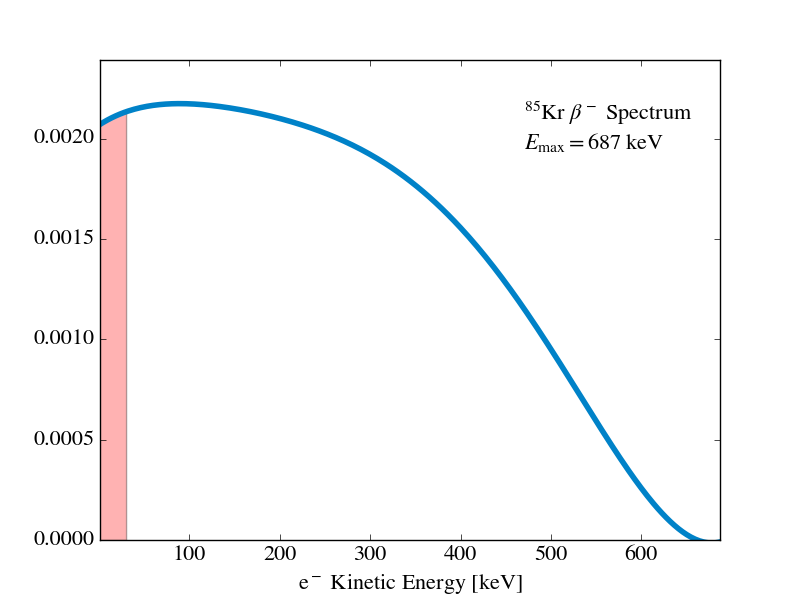
\includegraphics[width=0.7\textwidth]{kr85_beta_rates}
	\caption{The kinetic energy spectrum of electrons resulting from the $\beta^-$ decay of \ce{^{85}Kr} \cite{mantel1972beta}.  Note that roughly 3.1\% of decays are below 15 keV (shaded red region) which puts them inside the energy region of interest of WIMP searches.}
	\label{fig:kr85_beta_decay}
\end{figure}

% show multiple energy spectra of the beta decays from 
%https://ac.els-cdn.com/0020708X7290107X/1-s2.0-0020708X7290107X-main.pdf?_tid=259893f2-a843-11e7-9dfb-00000aacb35f&acdnat=1507039388_aef3096471a4defbd8b1c8a8198864c6

In liquid xenon based detectors, the two biggest sources of background beta decays are from \ce{^{85}Kr} and \ce{^{214}Pb}, which comes from the \ce{^{222}Rn} decay chain \cite{aprile2017first}.  Both of these background sources, which are discussed in more detail in \secref{sec:xe1t_er_kr85} and \secref{sec:xe1t_er_rn222},  must be carefully reduced, however other isotopes that $\beta^-$ decay have proven to be extremely useful for detector calibrations.  \ce{^{212}Pb}, from the decay chain of \ce{^{220}Rn} which can easily be introduced into TPCs,  has proven useful for calibrations since approximately 10\% of electrons have an energy less than 15 keV (the maximum energy is 570 keV) \cite{aprile2017results}.  \ce{^{220}Rn} as a calibration source will be discussed in more detail in \secref{sec:xe1t_er_rn222}.  Perhaps even more exciting for the low energy calibrations of electronic recoils is the use of tritium, which has a maximum energy of only 18.6 keV \cite{akerib2016tritium, aprile2017tritium}! \footnote{Molecular tritium ($\textrm{T}_2$) cannot be used because it adsorbs to surfaces very easily and the half-life of $\textrm{T}_2$ is 12.3 years.  Instead, tritiated methane ($\textrm{CH}_3\textrm{T}$) is used since this will not adsorb and can be easily removed.}  

\subsubsection{Photons}

Another source of electronic recoils in LXe comes from photons.  Photons, via photoelectric absorption, Compton scattering, or pair production, can create energetic electrons inside of a detector.  While pair production is not relevant in the energy range of interest, photoelectric absorption is one of the most tried and tested calibration tools for LXe (and other detectors) and electrons from Compton scatters can make up part of the background in WIMP searches since the energy of the electron can be arbitrarily low.

Photoelectric absorption is the process by which a photon is absorbed by an atom from which an electron is subsequently ejected (typically from the K shell).  This implies that the energy of the ejected electron is equal to the energy of the photon minus the binding energy.  However, the newly ionized atom will have a free electron bind with it, usually on a very short time scale, and an X-ray or auger electron will be emitted \cite{knoll2010radiation}.  Therefore the energy detected from photoelectric absorption will be very close to the initial energy of the photon.  Photoelectric absorption is the dominant mode of interaction up to a few hundred keV in most media, including xenon as can be seen in \figref{fig:photon_attenuation}.  

\begin{figure}[t]
	\centering
	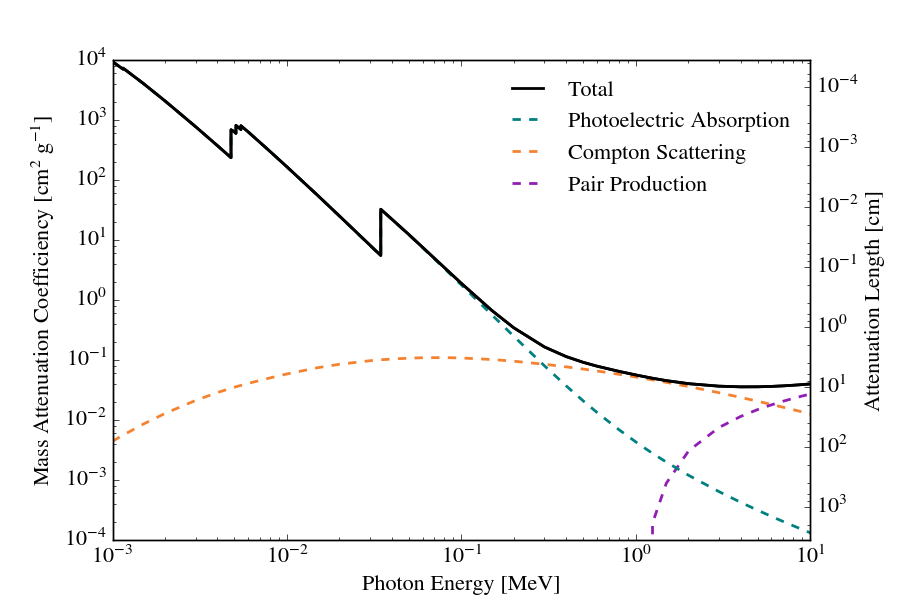
\includegraphics[width=0.95\textwidth]{photon_attenuation}
	\caption{The mass attenuation coefficient and the attenuation lengths for photons of different energies in liquid xenon \cite{berger8coll}.}
	\label{fig:photon_attenuation}
\end{figure}

Compton scattering is the process by which a photon interacts with an atomic electron resulting in the deflection of the photon at a specific angle and a transfer of energy to the electron.  The angle of the scattering completely describes the energy transferred to the electron.  Compton scattering is the dominant mode of interaction from a few hundred keV to a few MeV in most media, including xenon as can be seen in \figref{fig:photon_attenuation}.

\figref{fig:photon_attenuation} shows the mass attenuation coefficient of photons in LXe and the individual contributions of each process.  Because of xenon's high atomic number, all processes have very high attenuation coefficients.  This is valuable for background reduction since low energy photons are absorbed at the very edge of the detector (since their attenuation length is $<$ 1 cm) although it does make calibration with external gamma ray sources very difficult for large detectors.\footnote{This is the reason why many large scale LXe detectors are calibrated using internal sources now such as the beta emitters mentioned earlier and metastable activated xenon.}  Photons with an energy of a few hundred keV to a few MeV are most likely to Compton scatter and not be absorbed and have an attenuation length on the order of several centimeters which means that they will contribute to the background of LXe detectors at some level.
 

\subsubsection{Neutrons}

Neutrons can interact in liquid xenon mainly through three mechanisms: radiative absorption and inelastic scattering, which result in electronic interaction in the medium, and elastic scattering, which ultimately results in a nuclear recoil and will be discussed in \secref{sec:lxe_nr}.   The cross-sections of each of these mechanisms for xenon can be seen in \figref{fig:neutron_cross_section}.  Note that for almost all energies between 1 keV -- 10 MeV that elastic scattering is the dominant process.


\begin{figure}[t]
	\centering
	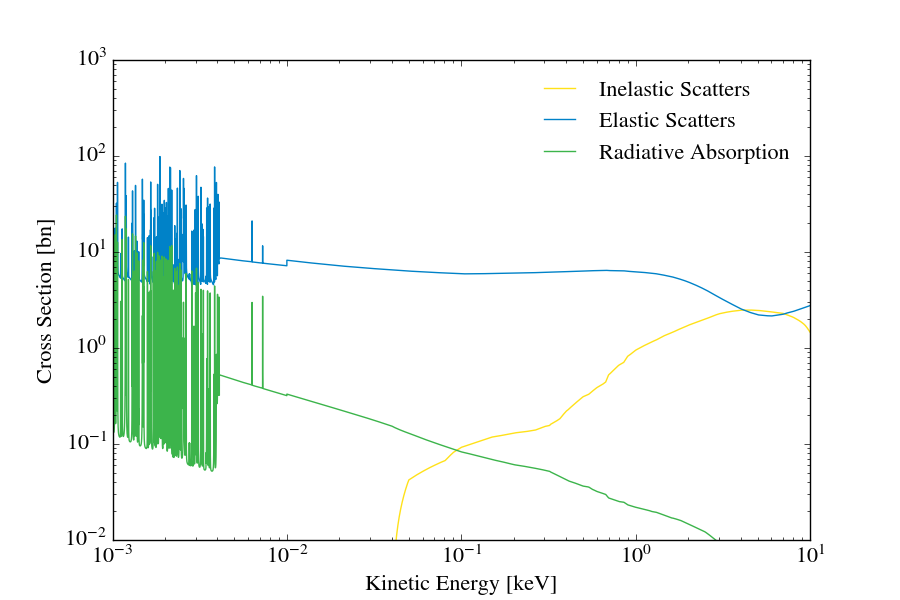
\includegraphics[width=0.95\textwidth]{neutron_cross_sections}
	\caption{The cross-sections of the three main interaction modes of neutrons in liquid xenon.  Note that elastic scattering is the dominant process for almost all energies in the range shown.  The data for each isotope of xenon is from \citeref{chadwick2011endf} and the figure shows the cross-sections weighted by abundance of each isotope in natural xenon.}
	\label{fig:neutron_cross_section}
\end{figure}


Radiative absorption is the absorption of neutrons by a nucleus.  The nucleus thus increases by one in mass number with atomic number staying the same.  Fortunately, since the isotopes of xenon that could be produced are not radioactive, with the exception of \ce{^{133}Xe} and \ce{^{135}Xe}, this process produces very little background.  \ce{^{133}Xe} and \ce{^{135}Xe} both result in short $\beta^-$ chains and will therefore result in electronic recoils inside of a detector.  With this said, for the neutron energies of background and calibrations in liquid xenon WIMP detectors, radiative absorption is largely irrelevant.

Inelastic scattering is the process by which a particle interacts with the atomic nucleus and kinetic energy is lost due to the excitation of the nucleus.  The excitation of the nucleus, also called \textit{activation}, is then followed by the nucleus decaying from this excited state back down to a stable state through the emission of a particle.  For xenon, there are two inelastic collisions of note:  an inelastic scattering with \ce{^{129}Xe} or \ce{^{131}Xe}.  A neutron scattering inelastically with \ce{^{129}Xe} can result in the nucleus being in an excited state with a 0.96 ns half-life that decays into gamma ray at an energy of approximately 40 keV or in an excited metastable state with a half-life of 8.8 days that results in a 197 keV photon followed by a 40 keV photon (the 40 keV photon is from the same very short lived state that the metastable state decays into) \cite{timar2014nuclear}.  A neutron scattering inelastically with \ce{^{131}Xe} can result in the nucleus being in a metastable state with a half-life of 11.84 days that decays emitting a 164 keV photon \cite{khazov2006nuclear}.   While these processes are not relevant for background considerations during a WIMP search, they are very useful when calibrating a detector since they each result in electronic recoils at a low and fixed energy.

There are three major sources of neutrons in dark matter experiments.  The first major source is from heavy elements in various detector components decaying via spontaneous fission resulting in neutrons with energies typically from 1 -- 10 MeV.  Neutrons also come from high-energy muons interacting with the rock and materials around the detector.  Finally, neutrons can be produced artificially using a neutron generator (typically either through a deuterium-deuterium reaction or deuterium-tritium reaction).  The first two sources of neutrons make up background in dark matter searches while the third source of neutrons is used to calibrate detectors (for both electronic and nuclear recoils).


\subsubsection{Neutrinos}

% https://arxiv.org/pdf/1512.07501.pdf
% largest source of neutrinos is the sun

Neutrinos can elastically scatter with electrons either via charged-current (exchange of W boson) or neutral-current (exchange of Z boson) interactions.  For electronic recoils, the main sources of neutrinos are from initial deuterium production and \ce{^7Be} reactions inside the sun (roughly 92\% and 7\% of the neutrino background, respectively) \cite{aprile2016physics}.  Like electronic recoils from beta decays, the kinetic energy of the recoiling electron will follow a spectrum where only very low energies ($\lesssim 15$ keV) are relevant.  Unlike other sources of electronic recoils, the solar neutrino background cannot be reduced and will scale with the size of the detector.

% example recoil spectrum shown in: https://journals.aps.org/rmp/pdf/10.1103/RevModPhys.59.505

%franarin2016reducing
\begin{figure}[t]
	\centering
	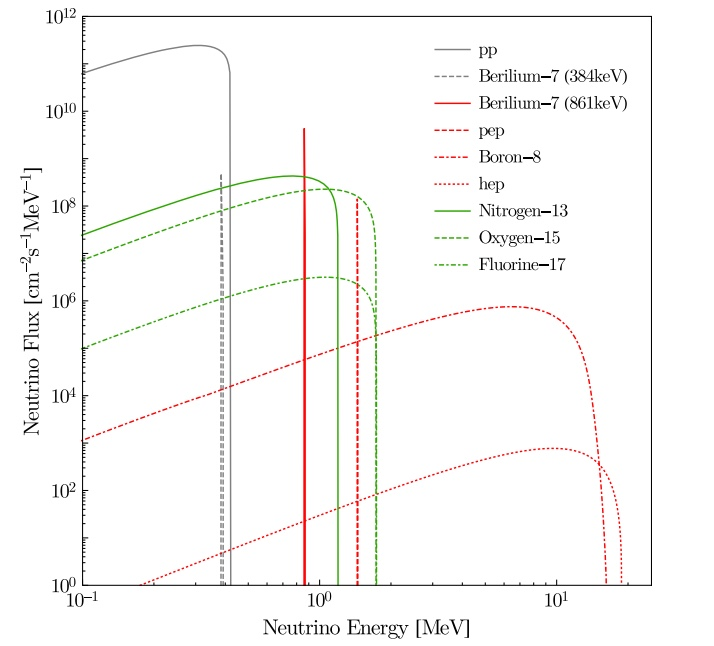
\includegraphics[width=0.7\textwidth]{solar_neutrino_flux}
	\caption{Solar neutrino fluxes from different processes assuming the BS05(OP) standard solar model.  Image Credit: \cite{franarin2016reducing}.}
	\label{fig:solar_neutrino_flux}
\end{figure}

\subsection{Observables Production for Electronic Recoils}
\label{sec:lxe_er_observables}

In \secref{sec:energy_deposition}, we discussed the modes by which charged particles deposit energy in LXe.  We will now quantify these observables production methods for electronic recoils under the assumption of an applied electric field.

As mentioned in \secref{sec:energy_deposition}, electronic recoils result in either excitation or the creation of electron-ion pairs.  Assuming the recoils occur in the presence of an electric field, we do not need to be concerned about quenching with respect to escape electrons (since these can be extracted by the electric field and ultimately measured).  Additionally, electronic recoils have relatively sparse tracks (as can be seen by their low stopping power in liquid xenon) \cite{aprile2006simultaneous} so it is expected that biexcitonic quenching will not play a large role in observables production.

Since there are no major forms of quenching, we can completely separate the energy deposited in the electronic recoil into excitons and electron-ion pairs.  Typically the total number of quanta (excitons and electron-ion pairs) is used to describe this relationship --- specifically, the average energy required to produce a single quanta.  For xenon, this value is $W = 13.7 \pm 0.2 \, \textrm{eV}$ \cite{dahl_thesis} and the relationship is given by \eqnref{eqn:w_value}.

\begin{equation}
        \label{eqn:w_value}
        N_q = \frac{\textrm{E}_{\textrm{ER}}}{W} = N_{\textrm{ex}} + N_{\textrm{ion}}
\end{equation}  

This relationship, while looking very simple, turns out to be extremely useful for calibrations in dual-phase xenon TPCs, as we will discuss in later chapters.  The breakdown of excitons to electron-ion pairs is simply described by the ratio of the two quantities such that we can define probabilities of a given quanta being an exciton or electron-ion pair.

\begin{equation}
        p_{\textrm{ion}} = \frac{1}{1 + \frac{N_{\textrm{ex}}}{N_{\textrm{ion}}}}, \, \, \, p_{\textrm{ex}} = 1 - p_{\textrm{ion}}
\end{equation}

The exciton-to-ion ratio, $\frac{N_{\textrm{ex}}}{N_{\textrm{ion}}}$, has been theoretically calculated to be 0.06 for sub-MeV electronic recoils \cite{takahashi1975average} however measurements and theoretical predictions have also suggested a value of $0.20 \pm 0.13$ \cite{doke2002absolute, aprile2007observation}.   

As mentioned previously, electron-ion pairs have a finite probability of recombining to form excitons and eventually producing a scintillation signal (as opposed to a charge signal).  While in the past this recombination probability was modelled using Birks' saturation law \cite{birks2013theory} for large tracks and the Thomas-Imel model \cite{thomas1987recombination} (which will be discussed in more detail for nuclear recoils) for short tracks, recently a great deal of work has gone into directly measuring recombination in liquid xenon and its potential fluctuations without the assumption of a model \cite{akerib2016tritium, aprile2017tritium}.  Recombination is simply inserted to the model of observables production as shown in \eqnref{eqn:recombination_er}.

\begin{equation}
        \label{eqn:recombination_er}
        N_{\textrm{ex}} \leftarrow N_{\textrm{ex}} + r N_{\textrm{ion}}, \, \, \, N_{\textrm{ion}} \leftarrow (1 - r) N_{\textrm{ion}}
\end{equation}

Following recombination in electronic recoils, these excitons and electron-ion pairs directly translate into the number of photons and electrons that are observable.

\begin{equation}
        \label{eqn:er_observables}
        N_{\gamma} = N_{ex}, \, \, \, N_e = N_{ion}
\end{equation}

\section{Nuclear Recoils in Liquid Xenon}
\label{sec:lxe_nr}

It is expected that WIMPs could potentially dissipate energy in xenon via elastic nuclear recoils so understanding these type of interactions is of crucial importance for WIMP direct detection experiments.  In this section, we will discuss the sources of nuclear recoils in liquid xenon based WIMP searches (besides potential WIMPs) and the observables production process for elastic nuclear recoils, which is substantially more complicated due to the nuclear and electronic quenching first mentioned in \secref{sec:energy_deposition}.



\subsection{Sources of Nuclear Recoils}

The two sources of nuclear recoils in liquid xenon based WIMP searches, besides potential WIMPs, are neutrons and neutrinos.   While neutrons are, as one would expect, the main background and calibration source in liquid xenon based WIMP searches, neutrinos are no longer negligible and, as detectors become more and more sensitive to lower cross-sections, will soon comprise an irreducible background of elastic nuclear recoils in detectors.  Understanding the sources of nuclear recoils in liquid xenon based WIMP direct detection experiments is very important since an underestimation of the background could lead to potential claims of a false WIMP signal since interactions would be indistinguishable on an event-by-event basis.

The sources discussed in this section are either considered to be background sources or calibration sources.  Calibration sources are sources that we knowingly introduce into the detector system such that we can measure the response of the xenon and our detector to these types of interactions.  They are controllable in such a way that we can both introduce them and remove them without consequence.  Calibration sources will not be present during dark matter searches.  Background sources, on the other hand, are sources that would be present when we are actively searching for WIMPs that we actively try to reduce but cannot be completely removed.

\subsubsection{Neutrons}

Electronic recoils from neutron scattering were discussed in \secref{sec:lxe_er} --- in this section we will focus on nuclear recoils from elastic scattering.  Elastic scattering is the process by which a particle interacts with the atomic nucleus and kinetic energy is conserved.  The recoiling nucleus then deposits its energy in the medium which can ultimately be detected.  Particles scattering elastically with nuclei is also called a nuclear recoil.  Of course, this process is not unique to neutrons but is the main mode of interaction for many massive particles (and hopefully WIMPs).  

Each of the sources of neutrons mentioned in \secref{sec:lxe_er}, spontaneous fission of heavy materials, high-energy muons, and artificially generated muons, can also result in nuclear recoils.




\subsubsection{Neutrinos}

Neutrinos can interact with both electrons, as discussed in \secref{sec:lxe_er}, and atomic nuclei, via coherent neutrino-nucleon scattering (CNNS).  The maximum energy of a recoiling nucleus is given by $E_{\textrm{r}}^{\textrm{max}} = \frac{2 E_{\nu}^2}{m_N + 2 E_{\nu}}$, where $m_N$ is the mass of the nucleus and $E_{\nu}$ is the energy of the neutrino.  This implies that neutrinos must have energies on the order of 10 MeV to cause nuclear recoils on the order of 1 keV.  Therefore, high energy neutrino sources like \ce{^{8}B} in the sun as well as neutrinos from supernovae and the atmosphere will contribute the most to the CNNS background in dark matter experiments.


\subsection{Observables Production for Nuclear Recoils}
\label{sec:xe_nr_observables}

We will now discuss the details of the observables production process for nuclear recoils that was generally outlined in \secref{sec:energy_deposition}.  Like electronic recoils, nuclear recoils can lead to the excitation or ionization of other xenon atoms.  However, unlike energetic electrons in liquid xenon, recoiling xenon atoms will also interact with other xenon nuclei.  This distinction is extremely important since energy can effectively be ``lost'' if the energy transferred during a collision is too low to cause excitation or ionization.  

Lindhard proposed a theory to describe this nuclear quenching in \citeref{lindhard1963integral}.  To describe the quenching of signals due to atomic motion, it is standard to work with the dimensionless energy given in \eqnref{eqn:dimensionless_energy}.

\begin{equation}
        \label{eqn:dimensionless_energy}
        \epsilon = 11.5 \left( \frac{E}{\textrm{keV}} \right) Z^{\sfrac{-7}{3}}
\end{equation}

Lindhard showed that at low velocities ($v < v_F$) the stopping power of a heavy ion in a medium is approximately given $S_e = k \epsilon^{\sfrac{1}{2}}$, where $k$ is a proportionality constant, assuming the Thomas-Fermi screening model.  Under the same assumptions, it can be shown that $k = 0.133 Z^{\sfrac{2}{3}} A^{-\sfrac{1}{2}}$, which would give $k \approx 0.165$ for xenon, although in his original paper Lindhard names the calculation of the proportionality factor as the largest source of uncertainty in the stopping power.  Shown in \eqnref{eqn:lindhard_electronic} is Lindhard's semi-empirical numerical solution for the fraction of the total energy that goes to electronic interactions for recoiling atoms.

\begin{equation}
        \label{eqn:lindhard_electronic}
        L(\epsilon) = \frac{k g(\epsilon)}{1 + k g(\epsilon)}, \, \, \, g(\epsilon) = 3 \epsilon^{0.15} + 0.7 \epsilon^{0.6} + \epsilon
\end{equation}

Note that $g(\epsilon)$ is not derived from first principles but is a fit to Lindhard's numerical solution from $\epsilon = 0.001 - 100$ (roughly 1 keV -- 100 MeV nuclear recoils for xenon).

Similar to observables production in electronic recoils, we assume that all energy that goes towards electronic interactions is converted into excitons and ions by way of the W value as is shown in \eqnref{eqn:quanta_nr}.

\begin{equation}
        \label{eqn:quanta_nr}
        N_q = \frac{L(E) E_{\textrm{NR}}}{W} = N_{\textrm{ex}} + N_{\textrm{ion}}
\end{equation}

As with electronic recoils, the split into excitons and ions can be defined by a single parameter, $\frac{N_{\textrm{ex}}}{N_{\textrm{ion}}}$.

\begin{equation}
        p_{\textrm{ion}} = \frac{1}{1 + \frac{N_{\textrm{ex}}}{N_{\textrm{ion}}}}, \, \, \, p_{\textrm{ex}} = 1 - p_{\textrm{ion}}
\end{equation}

Unlike electronic recoils, however, it is expected that $\frac{N_{\textrm{ex}}}{N_{\textrm{ion}}} \approx 1$ for nuclear recoils \cite{angle2011search, sorensen2011nuclear, lenardo2015global}.

RIVAL (Recoiling Ions in Various Atomic Liquids) simulations show that nuclear recoils, unlike electronic recoils, lose the majority of their energy in a large number of secondary tracks and have a short track size relative to electronic recoils.  With short tracks and with applied electric fields we can use the Thomas-Imel recombination model to describe the recombination of electrons and ions into excitons shown in \eqnref{eqn:ionization_production} \cite{dahl_thesis}.   The Thomas-Imel box model \cite{thomas1987recombination} begins by using the modified diffusion equation presented by Jaffe \cite{jaffe1913theory} with the assumptions that Coulomb forces are negligible, due to the high coefficient of polarization for xenon.  Jaffe's model is described by \eqnref{eqn:jaffe_recomb}.

\begin{equation}
        \label{eqn:jaffe_recomb}
        \frac{\partial N_{\pm}}{\partial t} = \mp u_{\pm} \bm{E} \cdot \bm{\nabla} N_{\pm} + D_{\pm} \nabla^2 N_{\pm} - \alpha N_+ N_-
\end{equation}

In \eqnref{eqn:jaffe_recomb} $N_{\pm}$ are the ion and electron charge distributions, $u_{\pm}$ are the ion and electron mobilities, and $\alpha$ is the recombination constant.  Thomas and Imel improved upon this model by making appropriate approximations for liquid xenon and argon: the diffusion rate is very small and ion drift is much slower than electron drift (3 -- 5 orders of magnitude).  These simplifications lead to the set of equations \ref{eqn:ti_diffeq}.

\begin{equation}
        \label{eqn:ti_diffeq}
        \begin{gathered}
                \frac{\partial N_+}{\partial t} = - \alpha N_+ N_- \\
                \frac{\partial N_-}{\partial t} = u_- E \frac{\partial N_-}{\partial z} - \alpha N_+ N_-
        \end{gathered}
\end{equation}

Assuming that the electron-ion pairs are isolated, that the initial distribution of ions and electrons uniformly populates a box of dimension $a$, and that $N_{ion}$ electron-ion pairs initially fill the box, we can solve equations \ref{eqn:ti_diffeq} to find the probability of recombination.

\begin{equation}
        \label{eqn:ti_recomb}
        r = 1 - \frac{\textrm{ln}(1 + N_{ion} \sigma)}{N_{ion} \sigma}, \, \, \, \sigma = \frac{\alpha}{4 a^2 \mu_- E}
\end{equation}

We redefine the number of excitons and electron-ion pairs following recombination in the same way as with electronic recoils.

\begin{equation}
        N_{\textrm{ex}} \leftarrow N_{\textrm{ex}} + r N_{\textrm{ion}}, \, \, \, N_{\textrm{ion}} \leftarrow (1 - r) N_{\textrm{ion}}
\end{equation}

Since nuclear recoils result in smaller and more dense tracks, we must also account for biexcitonic quenching.  Biexcitonic quenching occurs by the process outlined in \eqnref{eqn:biexcitonic_quenching}: two excitons collide ultimately leading to the formation of a single electron-ion pair.  This process effectively reduces the two potential photons to a single observable photon.  This electronic quenching is typically parameterized using the quenching term from Birks' saturation law, as shown in \eqnref{eqn:birks_quenching}, since one would expect that the density of excitons in a track to be proportional to the electronic stopping power \cite{mei2008model, tretyak2010semi, bezrukov2011interplay}. 

\begin{equation}
        \label{eqn:birks_quenching}
        f_B = \frac{1}{1 + \eta \frac{dE}{dx}} = \frac{1}{1 + \eta k \epsilon^{\sfrac{-1}{2}}}
\end{equation}

This quenching ultimately reduces the number of photons that will be observable in a given interaction, as shown in \eqnref{eqn:nr_observables}.

\begin{equation}
        \label{eqn:nr_observables}
        N_{\gamma} = N_{ex} f_B, \, \, \, N_e = N_{ion}
\end{equation}


% use following for biexcitonic quenching:
% https://ac.els-cdn.com/S0927650505000964/1-s2.0-S0927650505000964-main.pdf?_tid=e866eaac-a918-11e7-974f-00000aab0f6b&acdnat=1507131190_5bd95affa2fae24418f54ce96721ae8a
% https://arxiv.org/pdf/0712.2470.pdf
% https://ac.els-cdn.com/S0927650511001289/1-s2.0-S0927650511001289-main.pdf?_tid=baf2e1c0-a922-11e7-a7e2-00000aacb35d&acdnat=1507135409_d72980a38a6fbe81c7b4585e9dae6c97


\section{Dual-Phase Time Projection Chambers}
\label{sec:lxe_tpc}

Having discussed how different types of particles deposit their energy in liquid xenon, we can now discuss dual-phase xenon time projection chambers (TPCs), the leading detector type in the search for WIMPs, and how they identify interaction types and reconstruct the position and energy of interactions in a TPC.



\subsection{Operating Principle}
\label{sec:tpc_operating_principle}

On an interaction-by-interaction basis, the goal of dual-phase xenon TPC is three-fold: determine the type of the interaction (nuclear or electronic recoil), determine the energy of the interaction, and determine the position of the interaction.  While we will discuss in more detail how each of these goals is achieved in a TPC, it is important to understand how the observables are extracted from the liquid xenon.  

For both nuclear and electronic recoils, an interaction in the liquid xenon with an applied electric field results in both photons and free electrons.  The number of photons are measured by using photomultipler tube (PMT) arrays at the top and bottom of the detector.  These PMTs convert the light signal into a proportional charge signal that can be read by a standard digitizer.  This prompt scintillation signal is referred to as the S1 of the interaction.  The electric field that is applied vertically in the detector is used to extract the free electrons from the interaction site and to the liquid-gas boundary in the detector.  An additional electric field is applied to extract the electrons from the liquid and to accelerate the electrons through the gas, exciting xenon atoms that lead to secondary scintillation photons in the process.  This process occurs at a time directly related to the depth of the interaction in the liquid (discussed in more detail in \secref{sec:xe_pos_rec}).  This secondary scintillation process, which is proportional to the number of electrons extracted from the interaction site, is referred to as the S2 of the interaction.  This entire process is depicted in \figref{fig:tpc_principle} and will be discussed in significantly more detail throughout the remainder of this chapter.

\begin{figure}[t]
	\centering
	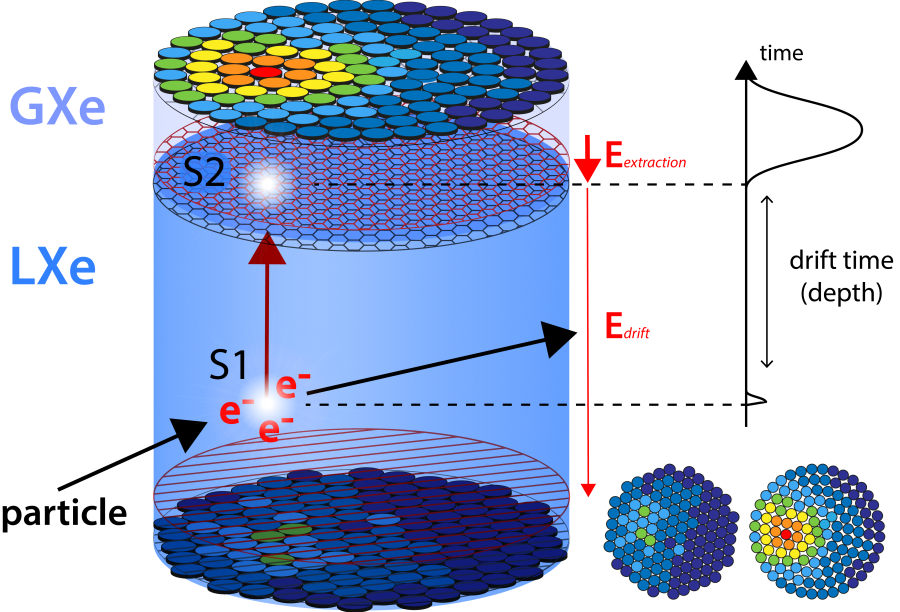
\includegraphics[width=0.99\textwidth]{tpc_principle}
	\caption{An example of an interaction in a dual-phase liquid xenon time projection chamber.  The interaction produces both scintillation light and free electrons.  The light is promptly detected by the PMT arrays at the top and bottom of the detector while the free electrons are drifted to the liquid-gas interface (maroon arrow) where they are extracted and accelerated through the gaseous xenon.  This acceleration through the gaseous xenon causes secondary excitations that result in more scintillation light that is detected by the PMT arrays.  The time difference between these interactions can be used to extract the depth of the interaction while the PMT hit patterns for the secondary signal can be used to find the interactions position in the transverse plane.}
	\label{fig:tpc_principle}
\end{figure}


\subsubsection{Reconstructing Interaction Type}

Since the most basic function of these TPCs is to search for WIMPs via elastic nuclear recoils, it becomes crucially important to be able say what is likely background (electronic recoils) and what is a potential signal (nuclear recoils).  Without this type of discrimination, searches are limited to counting techniques like those discussed in the first chapter.  Since the electronic recoil background rate is typically several orders of magnitudes larger than the nuclear recoil background, an experiment that can discriminate between the two interactions will be significantly more sensitive than a similar detector that is not.

As mentioned throughout this chapter, even though the energy deposition processes of electronic and nuclear recoils are similar they are far from identical.  These differences in track structure and interaction cross-sections lead to very large discrepancies in the amount of charge produced in an interaction relative to the amount of light produced at a given field.   For energies relevant to the WIMP search, the relationship shown in \eqnref{eqn:lxe_disc} holds for electronic and nuclear recoils and can be used to discriminate between them.  \figref{fig:xe1t_disc} shows this difference between electronic and nuclear recoils for XENON1T with a drift field of $116.7 \pm 7.5  \,\sfrac{\textrm{V}}{\textrm{cm}}$ \cite{aprile2017first}.

\begin{equation}
        \label{eqn:lxe_disc}
        \left( \frac{\textrm{S2}}{\textrm{S1}} \right)_{\textrm{ER}} > \left( \frac{\textrm{S2}}{\textrm{S1}} \right)_{\textrm{NR}}
\end{equation}

\begin{figure}[t]
	\centering
	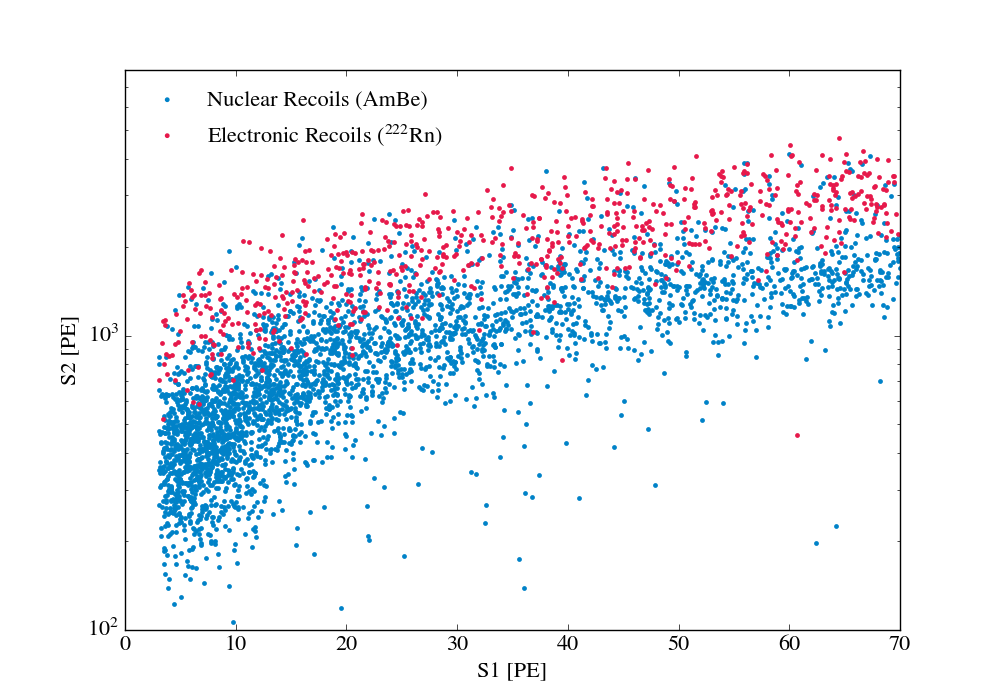
\includegraphics[width=0.99\textwidth]{xe1t_disc}
	\caption{Low energy electronic and nuclear recoils in liquid xenon.  Note that for a given S1 that the S2 for electronic recoils are usually significantly higher than the corresponding S2 for nuclear recoils.  The nuclear recoils are from an americium-beryllium (AmBe) source while the electronic recoils are from the \ce{^{222}Rn} decay chain that results in a $\beta^-$ emission with a maximum energy of 1.02 MeV.}
	\label{fig:xe1t_disc}
\end{figure}

This difference in the ratio of charge to light can actually be enhanced further: while $\frac{\textrm{S2}}{\textrm{S1}}$ for nuclear recoils has little to no dependence on the electric field applied in the TPC, $\frac{\textrm{S2}}{\textrm{S1}}$ for electronic recoils is heavily dependent on the electric field \cite{aprile2006simultaneous, goetzke2016measurement}, as can be seen in \figref{fig:field_dependence_nr_er}.  Therefore, the discrimination power between the two types of interactions can be increased by increasing the electric field used in the TPC.

\begin{figure}[t]
	\centering
	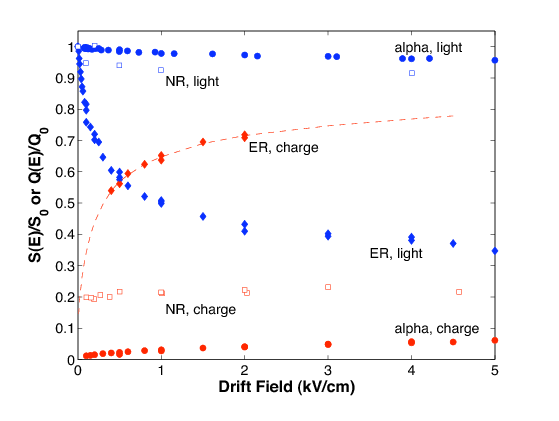
\includegraphics[width=0.85\textwidth]{field_dependence_nr_er}
	\caption{The field dependence of scintillation and ionization yield in liquid xenon for 122 keV electronic recoils and 56.5 keV nuclear recoils.  In blue are the light yields of interactions at a given field relative to the light yield with no applied electric field.  In red are the charge yields of interactions relative to the charge yield assuming no recombination.  Image Credit: \citeref{aprile2006simultaneous}}
	\label{fig:field_dependence_nr_er}
\end{figure}


\subsubsection{Reconstructing Energy}

A significant portion of this chapter was dedicated to understanding the production process of the observable photons and electrons in liquid xenon with an applied electric field.  With a perfect understanding of the observables production process and the detector effects, one could reconstruct the probability distribution for the energy of an event.  The reason you could not say the energy precisely, even with a perfect understanding of the physical processes described and the detector physics,  is because there is an associated smearing at each stage in the observables process -- in other words, two nuclear recoils depositing 10 keV at the same position in the detector will not produce exactly the same measured event each time.  

However, even being able to approximate the energy of an event is extremely important.  More precisely, an understanding of the process between energy deposition to the readout of observables is essential for the most sensitive dark matter searches.  The reason for this is because all predicted signals in the detector, including both background and potential WIMP signals, have a predictable energy spectrum.  Therefore, we can not only predict how many electronic and nuclear recoils there should be but we can also say \textit{where} they should be in an S1 and S2 spectrum.  As a concrete example, we expect the nuclear recoil background to fall off exponentially with increasing energy.  Therefore, an excess of events at high energies is more significant (or indicates a misunderstanding regarding the background) than an excess of events at low energies.


\subsubsection{Reconstructing Position}
\label{sec:xe_pos_rec}

An additional piece of information that proves to be very useful that can be extracted from TPCs is the the position of an event.  As mentioned earlier, an approximately uniform electric field is applied in the TPC to extract the electrons created in an interaction from the vertex to the liquid-gas interface where they will produce the secondary signal, the S2.  Of course, the scintillation light from the interaction is measured extremely quickly (on the order of nanoseconds such that we approximate the delay as zero) so the S1 can be used as the start of a timer that ends with the S2.  This drift time can then be used to reconstruct the depth of the interaction since the electron will travel with a constant velocity through the liquid xenon as given by $v_d = \mu E$, where $v_d$ is the drift velocity, $\mu$ is the mobility of electrons in liquid xenon, and $E$ is the electric field applied.   This analysis to determine the depth is shown on the right side of \figref{fig:tpc_principle}.

 \begin{figure}[t]
	\centering
	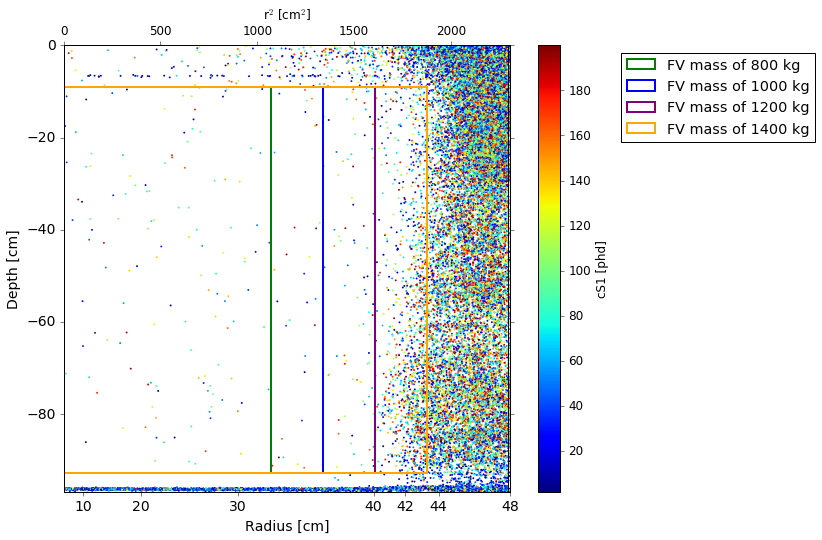
\includegraphics[width=0.99\textwidth]{tpc_pos_rec}
	\caption{The positions of all events during the first science run of XENON1T.  Notice that the overwhelming majority of events occur at the very edge of the detector and can be removed using a fiducial volume.}
	\label{fig:tpc_pos_rec}
\end{figure}

As mentioned earlier in this chapter, the stopping power for different charged particles in liquid xenon is high enough such that interactions will be stopped in $\lesssim 10 \, \mu \textrm{m}$.  Diffusion for electrons in liquid xenon is also small: even assuming a very large drift time of 1 ms, the expected transverse diffusion is on the order of $\sqrt{D_t t_d} \sim$ 20 mm so the electrons should still be very localized when arriving at the liquid-gas interface.  Once these electrons are accelerated through the gas layer they create the secondary photons (S2), which are then detected using the PMT arrays at the top and the bottom of the detector.  The hit pattern of the PMT arrays, specifically the top array because of its proximity, can be used to approximate the location of extraction at the liquid-gas interface, which should be a very good approximation of the position at the depth found using the drift time.  The PMT hit patterns are shown on the bottom-right of \figref{fig:tpc_principle}.

The three-dimensional location of an event inside a detector proves to be very important for WIMP searches.  To understand why, it is useful to consider a WIMP event in a detector.  Since the cross-section of the WIMP is so small, one would expect two features in a WIMP event: it would only scatter a single time and it could scatter anywhere in the liquid xenon with equal probability.  However, this is very different from almost all of our external background sources (the exception, of course, being neutrinos) - both external gamma, beta, and neutron sources that emit particles into the liquid xenon are expected to lose energy through multiple scatters, which can easily be identified and removed by observing multiple S2 peaks (called a \textit{multiple scatter cut}), and/or are expected to travel only a short distance before depositing all of their energy.  The latter effect can be seen in \figref{fig:tpc_pos_rec}, taken from XENON1T's first science run, which shows that the overwhelming majority of events occur at the very edges of the TPC.  One can then remove these events by making a \textit{fiducial volume cut} that removes all events not within a certain distance from the center of the detector --- four of these potential fiducial volume cuts are shown in \figref{fig:tpc_pos_rec}.  By using a multiple scatter cut and a fiducial volume cut, it is straightforward to remove almost all of the external background events, although it is important to note that this will not remove events from internal sources such as \ce{^{85}Kr} or \ce{^{222}Rn} or events from neutrino interactions.  Additionally, by removing the edges of the TPC the expected rate of WIMPs will decrease linearly with the target mass excluded.  Therefore, the volume must be chosen carefully such that the gain from background exclusion outweighs the loss in the expected WIMP scattering rate.



\subsection{Detecting Observables}

In this section we will discuss the details of how the observables produced by an interaction, the light and charge, are actually measured in TPCs to produce \textit{waveforms} like the one shown in \figref{fig:tpc_waveform}.

 \begin{figure}[t]
	\centering
	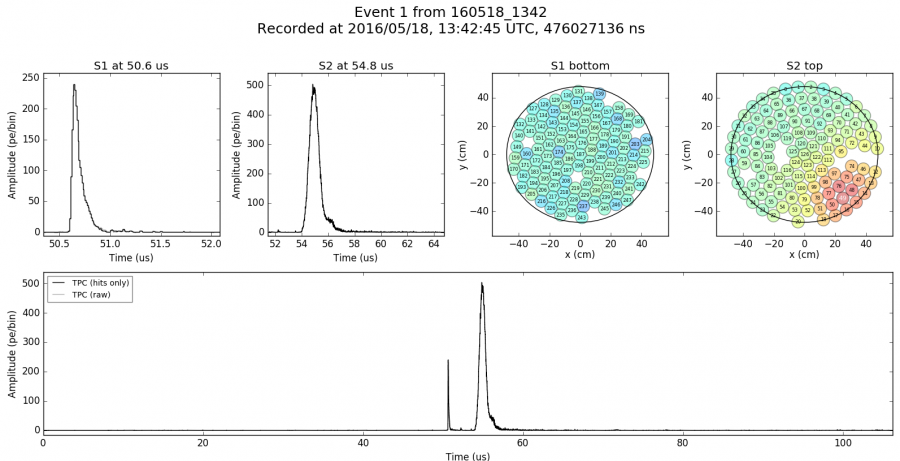
\includegraphics[width=0.99\textwidth]{tpc_waveform}
	\caption{The waveform of the first event seen by XENON1T.}
	\label{fig:tpc_waveform}
\end{figure}


\subsubsection{Detection of Scintillation Photons: S1}

The excited xenon dimers, excimers, decay very quickly (on the order of 10 ns) and produce 178 nm photons regardless of the interaction type.  These photons can be detected by the use of photomultiplier tubes (PMTs) that are designed to have peak efficiency for UV light.  In TPCs, the PMT arrays are placed at the top and bottom of the detector, as shown in \figref{fig:tpc_principle}, but cannot be placed around the sides of the TPC as the high voltage of the PMTs will prevent the electric field used to drift the electrons from being uniform in the vertical direction.  Because of this, light will typically reflect off of multiple surfaces before reaching the face of the PMT.  Since detectable light is lost during reflections, the position of the event will be important in understanding how much of the initial light is likely to be detected (with events closer to the PMTs and towards the center having a high detection efficiency than events near the edge of the TPC).  There is also an efficiency loss in the PMTs themselves since only roughly a third of photons that reach the photocathode of the PMT produce a signal --- this efficiency is referred to as the \textit{quantum efficiency} (QE).  These losses lead to roughly 90\% of light from an interaction not being detected!\footnote{Because of this large loss of scintillation light, a great deal of effort has gone into choosing and preparing material for the TPC to maximize the reflectivity \cite{silva2009reflectance, haefner2017reflectance, neves2017measurement}.}  

The main function of a PMT is to convert light signals into electrical signals, which can subsequently be digitized.  A schematic of a photomultiplier tube is shown in \figref{fig:tpc_pmt}.  When light shines upon the PMT window, there is a probability defined by the quantum efficiency that an electron is emitted by the photoelectric effect --- this electron is called a photoelectron.  This photoelectron is then guided and accelerated by an electric field to a stage of dynodes by which the initial electron produces secondary electrons at each stage in the chain.  The electrons reaching the end of the stage will be proportional to the initial number of photoelectrons and result in a current that can be digitized.  

 \begin{figure}[t]
	\centering
	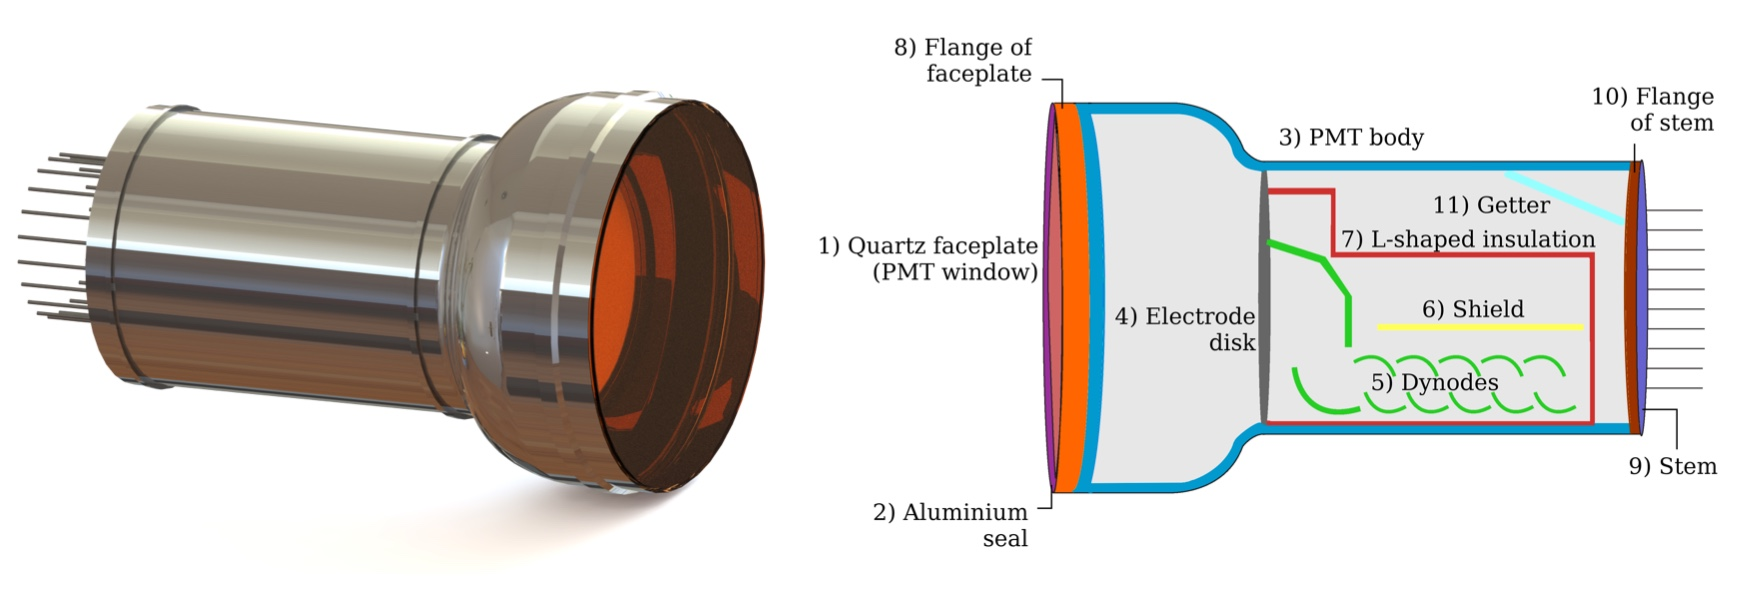
\includegraphics[width=0.99\textwidth]{tpc_pmt}
	\caption{The Hamamatsu R11410 PMT and a schematic illustration of its various components.  Image Credit: \citeref{aprile2015lowering}.}
	\label{fig:tpc_pmt}
\end{figure}

Since both the dexcitation of the excimers and the photomultiplication are both very fast processes (on the order of 10 ns), the S1 signal is considered to be a prompt signal.  This is very different from the S2 signal which will have a long delay (on the order of tens to hundreds of microseconds) depending on the depth of the interaction in the liquid xenon and the strength of the applied drift field.


\subsubsection{Detection of Ionization Electrons: S2}
\label{sec:tpc_s2_sig}

The S2 signal is a result of the electrons that do not recombine with an ion that was also created in the interaction.  These electrons are drifted using an approximately uniform vertical electric field to the liquid-gas interface.  Then, using a second electric field typically much stronger than the drift field (thousands of V/cm compared to hundreds), they are extracted from the liquid and accelerated through the gas, as shown in \figref{fig:tpc_principle}.  The accelerated electrons will create xenon excimers while being accelerated through the gas which will result in our secondary light signal that can be detected by PMTs.

The constant electron drift through the medium is actually an average over a series of many accelerations and decelerations.  The electrons are accelerated by the electric field and quickly lose energy in the liquid xenon through elastic scatters \cite{atrazhev2005electron}.  While this complicated series of interactions on a macro scale is quite simple, there is a complicating factor: electrons drifting through the liquid can be absorbed by electronegative impurities in the xenon, the most common of which is oxygen.  This process can also be examined from a larger scale and we can actually describe it with a single parameter: the so-called \textit{electron lifetime}.  The probability that an electron is not absorbed while drifting in the xenon is described in \eqnref{eqn:tpc_electron_lifetime}.

\begin{equation}
        \label{eqn:tpc_electron_lifetime}
        P(z) = \frac{1}{\tau_{e^-}} e^{-\frac{z}{v_d \tau_{e^-}}}
\end{equation}

In \eqnref{eqn:tpc_electron_lifetime}, z is the vertical distance between the electron and liquid-gas interface, $v_d$ is the drift velocity, and $\tau_{e^-}$ is the electron lifetime.  The xenon in a TPC must be constantly cleaned of these electronegative impurities to maintain a reasonable electron lifetime which proves to be technically challenging.  However, measuring the electron lifetime is relatively straight-forward.  The basic idea is that you look at an electronic recoil of known energy (the electronic recoil resulting from the decay of \ce{^{83m}Kr}, for example) and look at the S2 signal as a function of depth.   Since the light produced in the gaseous xenon is proportional to the number of electrons, one should see an exponential decrease in the size of the S2 as a function of depth according to \eqnref{eqn:tpc_electron_lifetime}.  An example of this type of electron lifetime measurement and the resulting exponential fit to the S2 size is shown in \figref{fig:tpc_electron_lifetime}.  As detectors grow in size it is critical that they are still able to clean the xenon of the increased level of impurities still since a low electron lifetime results in a large reduction in signal and smearing in S2 (which reduces discrimination power).

 \begin{figure}[t]
	\centering
	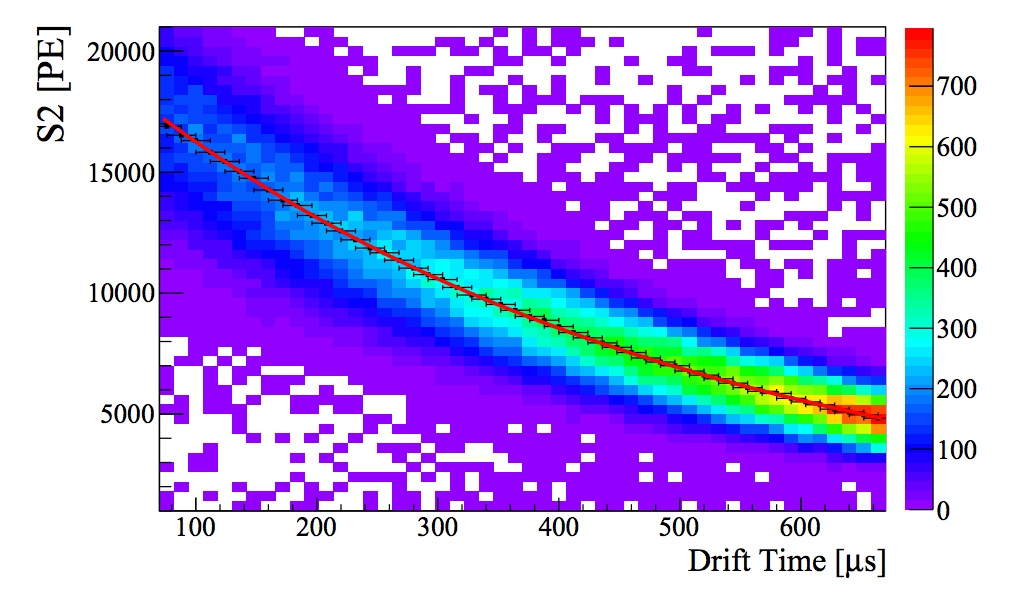
\includegraphics[width=0.99\textwidth]{tpc_electron_lifetime}
	\caption{An example of an electron lifetime analysis from XENON1T.  In this analysis, the 41 keV \ce{^{83m}Kr} electronic recoil is used and the decay's S2 signal size is plotted versus drift time (a proxy for depth).  Image Credit: \citeref{aprile2017xenon1t}.}
	\label{fig:tpc_electron_lifetime}
\end{figure}

Finally, the number of excitations produced in the gaseous xenon will be proportional to the number of electrons accelerated through.  The resulting number of photons for a single electron approximately follows a Gaussian distribution.  The mean of this Gaussian is referred to as the \textit{gas gain}.  Therefore, the number of electrons from the interaction can be inferred by looking at the number of photons detected by the photomultiplier tubes.  The response of the TPC to a single electron accelerated through gaseous xenon can also be measured in a relatively simple manner by looking at single electrons that drift to the liquid-gas interface (these single electrons often come from the photoionization of the stainless steel grids used to produce the drift field in the TPC).  This method is described in more detail in \citeref{aprile2014observation}, as well as in \secref{sec:xe1t_gas_gain} and \secref{sec:nerix_gas_gain}.  An example of this analysis is shown in \figref{fig:tpc_gas_gain}.

 \begin{figure}[t]
	\centering
	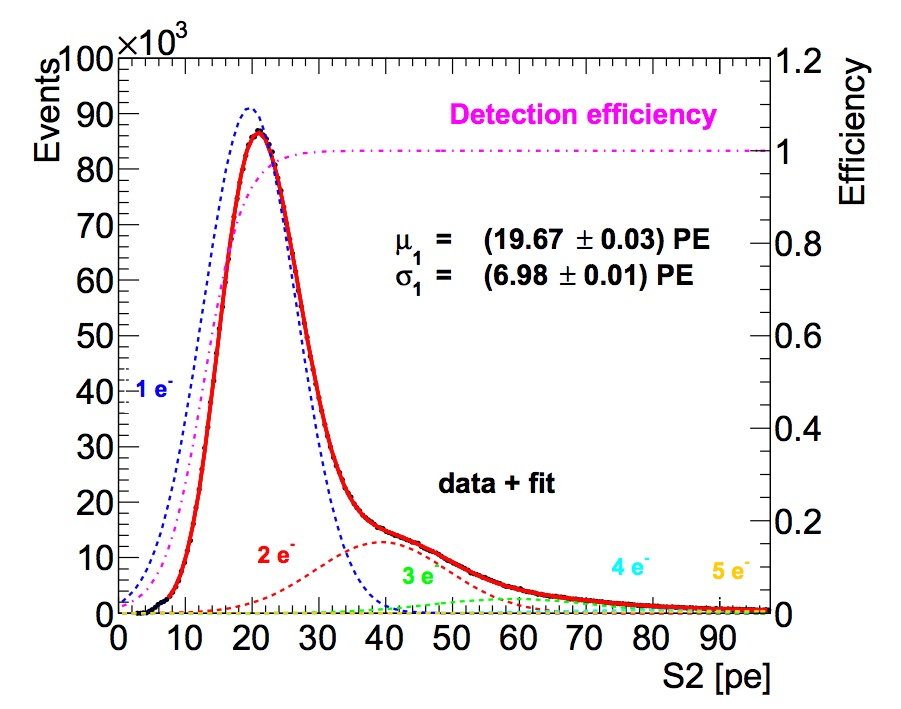
\includegraphics[width=0.8\textwidth]{tpc_gas_gain}
	\caption{An example of a gas gain analysis from XENON100.  This fit was performed using electrons from photoionization of metal inside of the detector.  Image Credit: \citeref{aprile2014observation}.}
	\label{fig:tpc_gas_gain}
\end{figure}


